\documentclass[a4paper,12pt]{article}
\usepackage[utf8]{inputenc}
\usepackage{amsmath}
\usepackage{graphicx}
\usepackage{listings}
\usepackage{caption}
\usepackage{float}
\usepackage{tikz}
\usepackage{pgfplots}
\pgfplotsset{compat=1.18}
\usepackage{longtable}
\usepackage{pgfplots}
\usepackage{xcolor}
\lstdefinestyle{mystyle}{
    keywordstyle=\color{blue},       % kolor słów kluczowych
    numberstyle=\tiny\color{gray},   % kolor numerów linii
    basicstyle=\ttfamily\footnotesize, % styl podstawowy
    breaklines=true,                 % łamanie długich wierszy
    captionpos=b,                    % pozycja podpisu
    numbers=left,                    % numery linii po lewej stronie
    numbersep=1pt,                   % odstęp numerów linii
    showspaces=false,                % nie pokazuj spacji
    tabsize=2                        % rozmiar tabulacji
}
\lstset{style=mystyle}

\title{Analiza Algorytmów}
\author{Ksawery Józefowski\\Politechnika Wrocławska}
\date{\today}

\begin{document}

\maketitle

\tableofcontents
\newpage

\section{Wstęp}
W ramach analizy zaimplementowano i przetestowano trzy algorytmy: 
\begin{itemize}
    \item Algorytm znajdowania najdłuższego wspólnego podciągu (LCS),
    \item Algorytm wyboru aktywności,
    \item Algorytm cięcia pręta.
\end{itemize}
Każdy algorytm został zaimplementowany w różnych wersjach: rekurencyjnej, iteracyjnej i dynamicznej. Celem analizy było porównanie ich efektywności i złożoności czasowej.

\section{Fragmenty kodów}
\subsection{LCS}
Algorytm LCS (Longest Common Subsequence) pozwala znaleźć najdłuższy wspólny podciąg dwóch sekwencji znaków. Jest używany w takich dziedzinach jak bioinformatyka czy porównywanie tekstów. Poniżej przedstawiono implementację rekurencyjną tego algorytmu:
\begin{lstlisting}[language=C++]
int LCS_Rec(char X[], char Y[], int m, int n, int c[MAX_M + 1][MAX_N + 1]) {
    if (m == 0 || n == 0) return 0;
    if (X[m - 1] == Y[n - 1]) {
        comparisons++;
        assignments++;
        c[m][n] = 1 + LCS_Rec(X, Y, m - 1, n - 1, c, assignments, comparisons);
    } else {
        comparisons++;
        assignments++;
        c[m][n] = max(LCS_Rec(X, Y, m - 1, n, c, assignments, comparisons),
                            LCS_Rec(X, Y, m, n - 1, c, assignments, comparisons));
    }
    return c[m][n];
}
\end{lstlisting}

\subsection{Algorytm wyboru aktywności}
Algorytm wyboru aktywności znajduje maksymalny zbiór niepokrywających się czasowo aktywności. Jest to problem klasyczny w optymalizacji, szczególnie w harmonogramowaniu zadań. Poniżej przedstawiono implementację dynamiczną tego algorytmu:
\begin{lstlisting}[language=C++]
void dynamicActivitySelector(Activity activities[], int n, int selected[], int& selectedCount) {
    int dp[n];
    std::sort(activities, activities + n, compare);
    dp[0] = 1;
    for (int i = 1; i < n; ++i) {
        dp[i] = 1;
        for (int j = i - 1; j >= 0; --j) {
            if (activities[i].start >= activities[j].finish) {
                dp[i] = std::max(dp[i], dp[j] + 1);
            }
        }
    }
}
\end{lstlisting}

\newpage
\subsection{Algorytm cięcia pręta}
Algorytm cięcia pręta (Rod Cutting) rozwiązuje problem maksymalizacji zysku przy cięciu pręta na kawałki o określonych długościach. Jest to klasyczny problem dynamiczny, stosowany w optymalizacji zasobów. Poniżej przedstawiono wersję Extended Bottom Up:
\begin{lstlisting}[language=C++]
void Bottom_Up_Cut_Rod(const int p[], int* r, int* s, int n) {
    r[0] = 0;
    for (int j = 1; j <= n; j++) {
        int q = -1;
        for (int i = 1; i <= j; i++) {
            if (q < p[i] + r[j - i]) {
                q = p[i] + r[j - i];
                s[j] = i;
            }
        }
        r[j] = q;
    }
}
\end{lstlisting}

\newpage
\section{Analiza i wyniki}
Porównano algorytmy pod względem liczby operacji i czasu wykonania dla różnych rozmiarów danych wejściowych.

\subsection{Tabele wyników}
\subsubsection{LCS}
\begin{longtable}{|c|c|c|c|c|c|}
\hline
Rozmiar danych & Algorytm & Porównania & Przypisania & Czas (ms) \\
\hline
1 & LCS (rekurencyjny) & 2 & 2 & 920 ns \\
1 & LCS (iteracyjny) & 7 & 10 & 1210 ns \\
\hline
10 & LCS (rekurencyjny) & 564 & 564 & 4700 ns \\
10 & LCS (iteracyjny) & 140 & 100 & 1500 ns \\
\hline
100 & LCS (rekurencyjny) & 7919 & 7919 & 254640 ns \\
100 & LCS (iteracyjny) & 1291 & 847 & 5080 ns \\
\hline
\caption{}
\label{tab:results}
\end{longtable}

\subsubsection{Cut Rod}
\begin{longtable}{|c|c|c|c|c|c|}
\hline
Rozmiar danych & Algorytm & Porównania & Przypisania & Czas (ms) \\
\hline
1 & Cut Rod & 1 & 1 & 50 ns \\
1 & MemorizedCutRod & 1 & 4 & 570 ns \\
1 & Bottom_UpCutRod & 1 & 4 & 180 ns \\
\hline
10 & Cut Rod & 1023 & 1023 & 6850 ns \\
10 & MemorizedCutRod & 100 & 76 & 1080 ns \\
10 & Bottom_UpCutRod & 55 & 31 & 360 ns \\
\hline
20 & Cut Rod & 1048575 & 1048575 & 7116060 ns \\
20 & MemorizedCutRod & 400 & 251 & 2190 ns \\
20 & Bottom_UpCutRod & 210 & 61 & 820 ns \\
\hline
\caption{}
\label{tab:results}
\end{longtable}

\newpage
\subsubsection{Activity Selector}
\begin{longtable}{|c|c|c|c|c|c|}
\hline
Rozmiar danych & Algorytm & Porównania & Przypisania & Czas (ms) \\
\hline
1 & ActivitySelector (rekurencyjny) & 1 & 4 & 1200 ns \\
1 & ActivitySelector (iteracyjny) & 2 & 5 & 33 ns \\
1 & ActivitySelector (dynamiczny) & 3 & 11 & 300 ns \\
\hline
10 & ActivitySelector (rekurencyjny) & 11 & 20 & 933 ns \\
10 & ActivitySelector (iteracyjny) & 15 & 14 & 133 ns \\
10 & ActivitySelector (dynamiczny) & 78 & 64 & 900 ns \\
\hline
100 & ActivitySelector (rekurencyjny) & 100 & 125 & 1366 ns \\
100 & ActivitySelector (iteracyjny) & 112 & 38 & 400 ns \\
100 & ActivitySelector (dynamiczny) & 5151 & 3371 & 34333 ns \\
\hline
\caption{}
\label{tab:results}
\end{longtable}

\subsection{Wykresy Wyników}
\subsubsection{Activity Selector}
\begin{figure}[H]
    \centering
    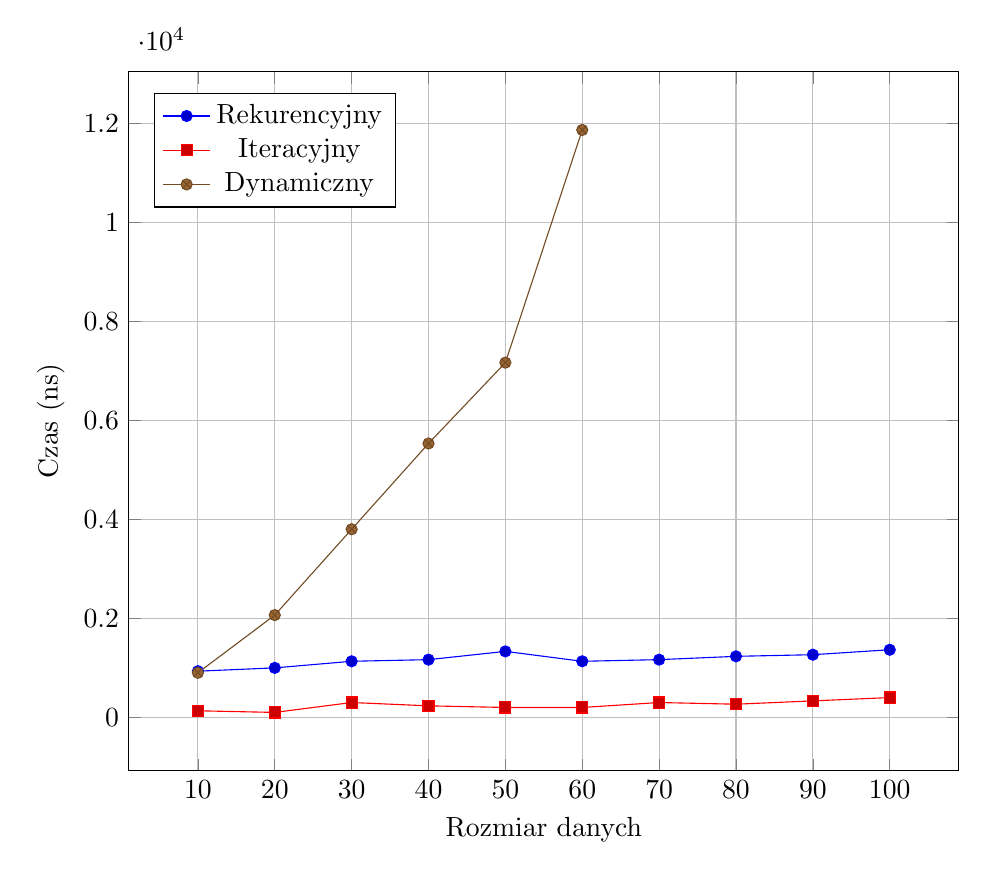
\begin{tikzpicture}
        \begin{axis}[
            width=\textwidth,
            xlabel={Rozmiar danych},
            ylabel={Czas (ns)},
            legend pos=north west,
            grid=major,
        ]
        \addplot coordinates {(10, 933) (20, 1000) (30, 1133 )  (40, 1166 )  (50, 1333 )  (60, 1133 )  (70, 1166 )  (80, 1233 )  (90, 1266 )  (100, 1366 )};
        \addplot coordinates {(10, 133) (20, 100) (30, 300 )  (40, 233 )  (50, 200 )  (60, 200 )  (70, 300 )  (80, 266 )  (90, 333 )  (100, 400 )};
        \addplot coordinates {(10, 900) (20, 2066) (30, 3800 )  (40, 5533 )  (50, 7166 )  (60, 11866 )};
        \legend{Rekurencyjny, Iteracyjny, Dynamiczny}
        \end{axis}
    \end{tikzpicture}
    \caption{Porównanie czasu wykonania algorytmów}
    \label{fig:execution_time}
\end{figure}

\subsubsection{Cut Rod}
\begin{figure}[H]
    \centering
    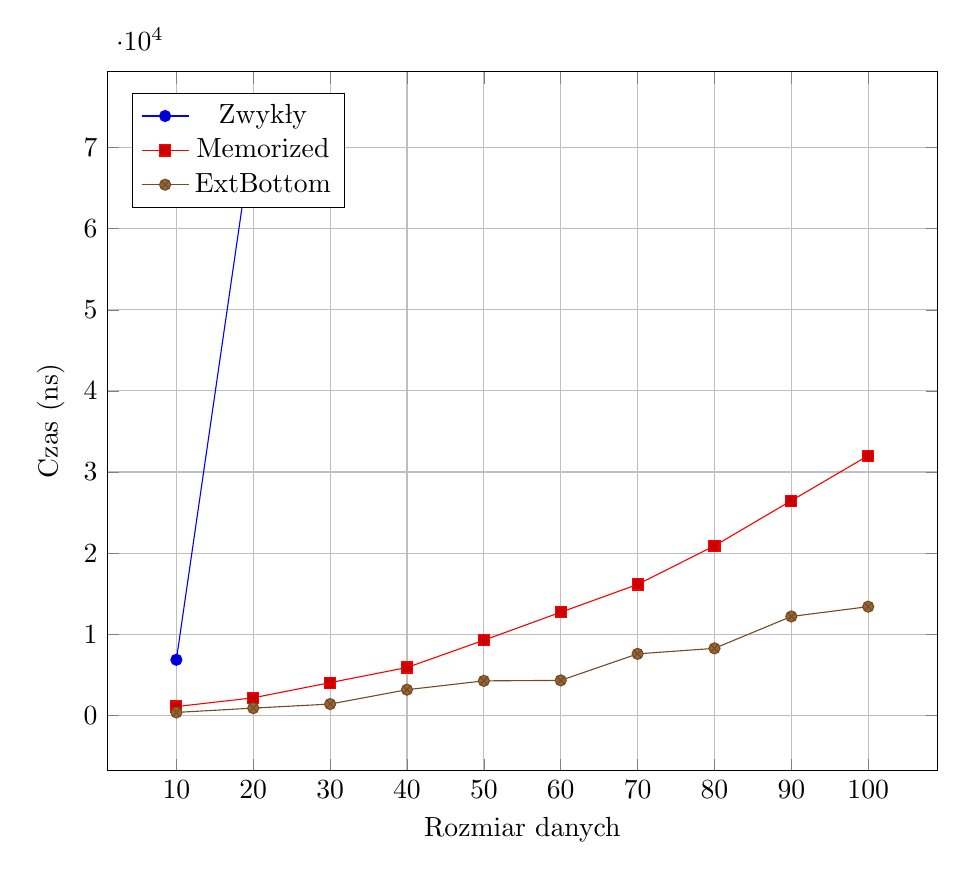
\begin{tikzpicture}
        \begin{axis}[
            width=\textwidth,
            xlabel={Rozmiar danych},
            ylabel={Czas (ns)},
            legend pos=north west,
            grid=major,
        ]
        \addplot coordinates {(10, 6850) (20, 72170)};
        \addplot coordinates {(10, 1080) (20, 2160) (30, 4030 )  (40, 5900 )  (50, 9260 )  (60, 12710 )  (70, 16140 )  (80, 20900 )  (90, 26470 )  (100, 32020 )};
        \addplot coordinates {(10, 360) (20, 890) (30, 1390 )  (40, 3160 )  (50, 4250 )  (60, 4310 )  (70, 7580 )  (80, 8260 )  (90, 12190 )  (100, 13400 )};
        \legend{Zwykły, Memorized, ExtBottom}
        \end{axis}
    \end{tikzpicture}
    \caption{Porównanie czasu wykonania algorytmów}
    \label{fig:execution_time}
\end{figure}

\subsubsection{LCS}
\begin{figure}[H]
    \centering
    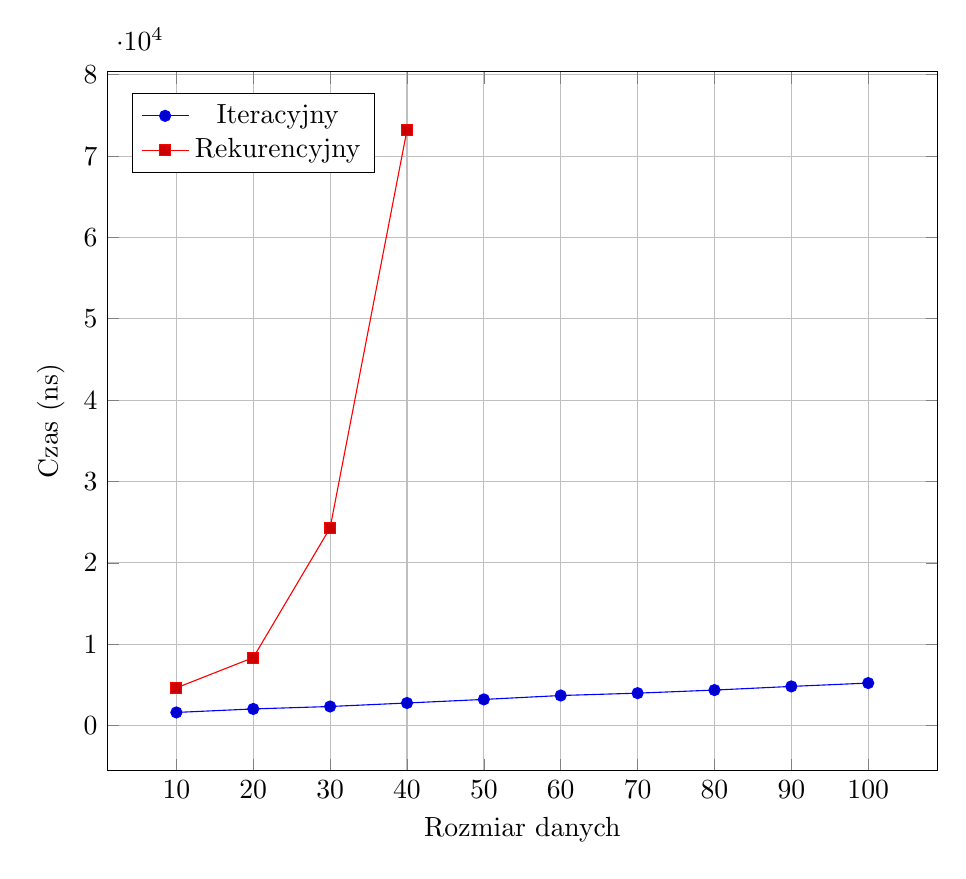
\begin{tikzpicture}
        \begin{axis}[
            width=\textwidth,
            xlabel={Rozmiar danych},
            ylabel={Czas (ns)},
            legend pos=north west,
            grid=major,
        ]
        \addplot coordinates {(10, 1600) (20, 2030) (30, 2330 )  (40, 2760 )  (50, 3200 )  (60, 3680 )  (70, 3970 )  (80, 4350 )  (90, 4800 )  (100, 5210 )};
        \addplot coordinates {(10, 4620) (20, 8342) (30, 24293 )  (40, 73214 )};
        \legend{Iteracyjny, Rekurencyjny}
        \end{axis}
    \end{tikzpicture}
    \caption{Porównanie czasu wykonania algorytmów}
    \label{fig:execution_time}
\end{figure}

\newpage
\section{Wnioski}

Na podstawie przedstawionych wyników i wykresów dotyczących trzech algorytmów: LCS, Cut Rod oraz Activity Selector, można wyciągnąć kilka istotnych wniosków:

\begin{itemize}
    \item \textbf{Algorytmy rekurencyjne vs. iteracyjne:}
    \begin{itemize}
        \item W przypadku algorytmu \textbf{LCS}, algorytm rekurencyjny wykazuje znacząco dłuższy czas wykonania niż algorytm iteracyjny. Wynika to z braku optymalizacji w wersji rekurencyjnej, która może prowadzić do nadmiernych obliczeń dla większych danych.
        \item W \textbf{Cut Rod}, wersja z pamięcią (MemorizedCutRod) jest wyraźnie szybsza od klasycznego algorytmu (Cut Rod), co wskazuje na korzyści płynące z zapamiętywania wyników podproblemów i unikania ich wielokrotnego obliczania.
    \end{itemize}
    \item \textbf{Algorytmy dynamiczne:}
    \begin{itemize}
        \item W przypadku algorytmu \textbf{Activity Selector}, wersja dynamiczna ma tendencję do wydłużania czasu obliczeń w porównaniu do wersji iteracyjnej, szczególnie dla większych rozmiarów danych. Mimo to, algorytmy dynamiczne są skuteczne w rozwiązywaniu problemów o większej złożoności.
        \item W \textbf{Activity Selector}, wersja iteracyjna jest zdecydowanie najszybsza, co może wynikać z prostszej implementacji i mniejszej liczby operacji wymaganych do rozwiązania problemu.
    \end{itemize}
    \item \textbf{Zależność czasu wykonania od rozmiaru danych:}
    \begin{itemize}
        \item W przypadku \textbf{LCS} i \textbf{Cut Rod}, czas wykonania algorytmów wzrasta w miarę zwiększania rozmiaru danych, co jest zgodne z oczekiwaniami dotyczącymi algorytmów o złożoności czasowej zależnej od rozmiaru wejścia.
        \item Dla algorytmu \textbf{Activity Selector}, wersja dynamiczna charakteryzuje się znacznie większym czasem wykonania w porównaniu do wersji rekurencyjnej i iteracyjnej, szczególnie przy większych rozmiarach danych, co sugeruje większą złożoność obliczeniową tego podejścia.
    \end{itemize}
\end{itemize}

\end{document}

